\documentclass[11pt]{article}
\usepackage{graphicx}
\usepackage{authblk}
\usepackage[utf8]{inputenc}
\graphicspath{/Users/georgeadams/Dropbox/005_ITP_projects/003 TPO/GIT_repo_TPOPROJECT/}


\title{Bayesian Analysis of TPO levels in Immune Thrombocytopenia}
\author[1,2]{\small George Adams}
\author[1,2]{\small Nichola Cooper}
\affil[1]{\footnotesize Imperial College London, Kensington, London SW7 2AZ}
\affil[2]{\footnotesize Hammersmith Hospital, Imperial College NHS Trust, London W12 0HS}



\date{July 2018}

\begin{document}

\maketitle

\paragraph{Introduction:} Thrombopoietin (TPO) is the main regulator of platelet production and TPO-mimetics are increasingly being used as treatment in immune thrombocytopenia. It is believed that TPO is largely synthesised in a constitutive manner and that platelets bind TPO via high-affinity receptors of their surface and remove TPO from the circulation. The current working hypothesis for platelet regulation by TPO is that when platelet counts go too low, TPO levels increase thus driving increased thrombopoeisis and vice versa (The `sponge theory') \cite{EtoLinkagemechanismsthrombocytopenia2016}. This hypothesis requires that their be a direct inverse relationship between platelet counts and TPO levels. Patients with ITP have been shown to have inappropriately low TPO levels, and are reported to have TPO levels approaching that of normal patients but at much lower platelet counts. It has been suggested that this reflects the high turnover of platelets during active ITP which accentuating the inverse relationship between TPO and platelets. To test the hypothesised relationship between TPO and platelets in ITP we measured TPO levels in a 67 patients with ITP. We used a bayesian regresssion to analyse the association between TPO and platelet counts. This approach allows us to infer TPO concentration over a range of different platelet counts and has been shown to be more accurate with smaller sample sizes than classical gaussian regression models \cite{GoldsteinBayesiananalysisregression1976}.


\paragraph{Methods:} 67 ITP patients had blood samples taken between May to November 2014 in an outpatients setting. Many of these patients had duplicated samples resulting in a in a total of 121 samples collected. Samples were collected in sodium citrate tubes, double spun to remove platelet fractions and then stored at -80°C within four hours of collection. Patients also had a full blood count measured at the time of collection. TPO levels measurements perfomed by quantitive sandwich enzyme immunoassay technique, used according to manufacturers instructions. Optical density values measured by microplate reader. For analysis, a bayesian regression model was used of (log-normalised) platelet count regressed against (log-normalised) TPO; $log(TPO) = alpha + beta*log(platelet)$. We used uninformative gaussian priors (mean 0, standard deviation 10) for the model. We predicted posteriors distributions for a range of different platelet counts (1 to 200) to determine how TPO concentrations in the blood changed over this range. Statistical analyses were performed using R.

\paragraph{Results:} Of the 121 samples collected, we excluded 30 which failed to show any TPO result, leaving 91 samples. We had positive repeat samples on many of these patients which indicated these zero values where due to laboratory assay failures rather than true absence of TPO. The TPO range was between 14-829.3pg/ml (normal range for health individual ~ 80pg/ml) and platelet counts ranged from 4 to 452 x$10^9/L$.  We predicted TPO distributions for platelet counts; 1 to 200. Figure 1A showes the infered distributions of TPO for platelet counts 10, 20, 30, 40, 50, 60, 70, 80, 90 and 100. The maximium a posteriori (MAP) estimates, which reflect the maximium point within the distribution were calculated for the different platelets counts (1 to 200). For platelet count of 1 the MAP was calculated at 410pg/ml (bayesian confidence interval, BCI; 200-804pg/ml). This declined sharply to 100pg/ml as the platelet count increased from 1 to 10x10$^9/L$. As the platelet count further increased up to 50$x10^9/L$ the TPO level stabilised to a MAP estimate of  As platelet counts increased the TPO level then declines in a non-linear manner (Figure 1B.) with the MAP estimate falling from 407pg/ml to approximately 100pg/ml (BCI 164 to 281 pg/ml) as platelet counts increased from 1 to 10$x10^9/L$. TPO levels continued to fall as with platelet counts rising from 10 to 50$x10^9/L$ at which point TPO levels were 37.5pg.ml (BCI 31 to 46pg/ml) and then declined much more slowly do approximately 16 pg/ml (BCI 11-21 pg/ml).

\paragraph{Conclusions:} Our study identified that in patients with ITP there is a clear non-linear correlation between platelet count and TPO level, with a flattening off of TPO levels at platelet counts between 50-100$x10^9/L$. Consistent with previous studies, TPO levels in ITP patients approached levels found in healthy individuals at much lower platelet counts. ITP patients with a platelet count 10$x10^9/L$ had TPO levels of approximately 100pg/ml which is similar to the expect levels seen in healthy individuals (approximately 120pg/ml, range 80 - 230pg/ml) \cite{SinghCirculatingthrombopoietinlevels2015}. However, this ITP patients as the platelet count increased to normal ranges, as patients went into remission, TPO levels also fell. As such, in patients in remission with platelet counts \geqlant150$x10^9/L$ TPO levels were only approximately 16pg/ml (range 11-21pg/ml), four-fold lower than healthy levels. Furthermore the fact that TPO levels changed only very slightly in our patients with platelet counts \geqslant50 is in opposition to the `sponge theory' of TPO regulation. These findings would be more consistent with failure in TPO production as opposed to excessive removal. This would also support the rationale for supplementation of TPO with TPO agonists in ITP, which clinically have been demonstrated to be highly effective.  \cite{WangEfficacysafetythrombopoietin2016}.


\begin{center}
 \begin{tabular}{||c c c c c||}
 \hline\hline
  ITP   & platelet count & MAP & LL & UL    \\
\hline\hline
 Platelet count & 1 & 410 & 200  & 804 \\
 \hline
 Patelet count & 10 & 100 &  75 & 151 \\
 \hline
 Platelet count & 50 & 37.5 & 31 & 46 \\
 \hline
 Platelet count & 200 & 16 & 11 & 21 \\ [1ex]
 \hline
\end{tabular}
\end{center}

\begin{figure}
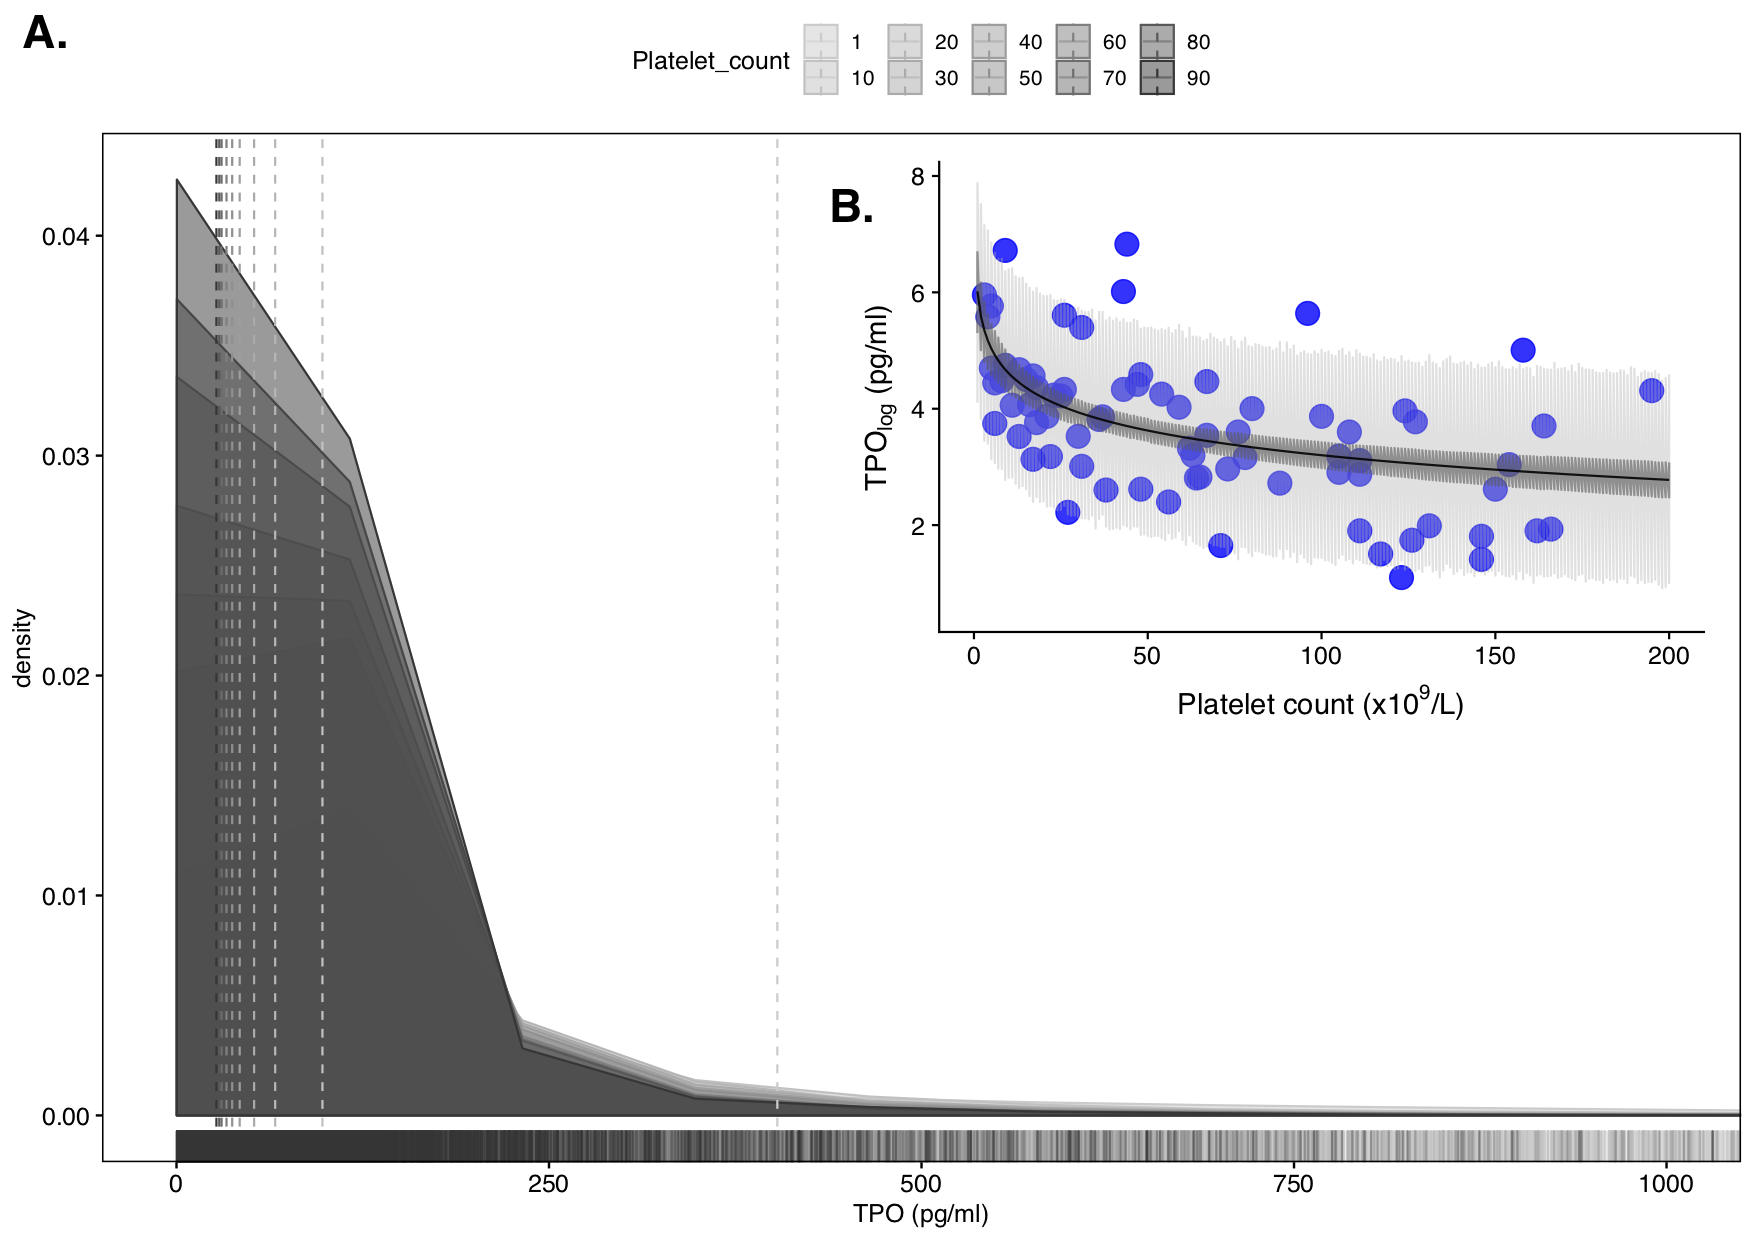
\includegraphics[]{ABSTRACT_v1_graph1.png}
\caption{A. Shows predicted TPO distributions for at different platelet counts ranging from 10 to 90. Dashed vertical lines represent median values for each distribution. B. LogTPO levels versus platelet counts showing individual patient results and the predicted non-linear assocaition produced by model. Darker shaded area is the 90\% bayesian confidence interval and the lighter shaded area around curve shows total predicted distribution width}
\end{figure}

\bibliographystyle{plain}
\bibliography{tpobib.bib}


\paragraph{}
\textbf{Total characters: 3800}


\end{document}
